\section{Rockwell B-1 Lancer}

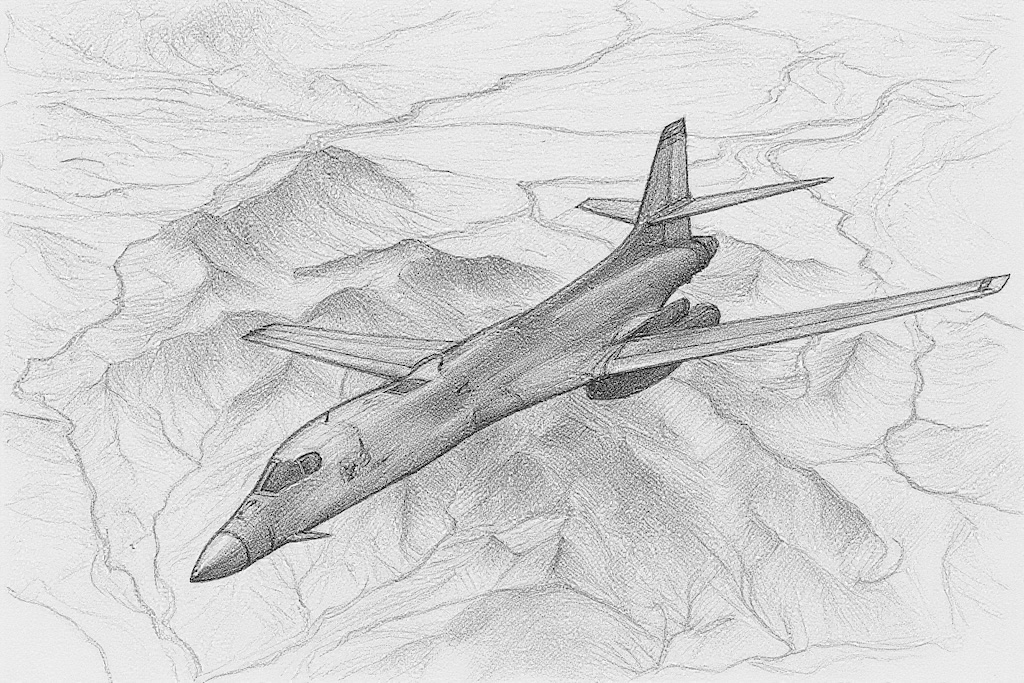
\includegraphics[width=\linewidth]{B-1B.jpg}

The Rockwell B-1 Lancer is a long-range strategic bomber. Although it is formally called the “Lancer,” informally it is referred to as the “Bone”.

\subsection{Versions}

\subsubsection{B-1A}

The aircraft was originally designed and developed as long-range, high-speed strategic nuclear bomber. However, the project was cancelled in 1977 to a large degree since it was thought that the B-52 with air-launched cruise missiles could provide an equivalent capability at a lower cost. The B-1A did not progress past the prototype stage.

\subsubsection{B-1B}

The B-1 was revived in the 1980s as a long-range conventional bomber with a secondary nuclear strike capability. Modifications gave lower radar cross-section and higher speed at low altitude, at the cost of much reduced speed at high altitude.

\subsection{Armament and Stores}

The B-1B has three internal bays. Each can carry a Conventional Bomb Module (CBM), a Multi-Purpose Rotary Launcher (MPRL), or a fuel tank. The forward two bays can be combined to carry a Common Strategic Rotary Launcher (CSRL). Each of these weapon racks has different load options.

Initially, armaments were limited to nuclear weapons and the Mk~82 500 lb and Mk~84 2000 lb BB. These options were expanded in a series of upgrades: the block C upgrade in 1997 added the ability to carry cluster BBs; the block D upgrade in 1998 added the GBU-31 JDAM BG; the block E upgrade in 2006 added the AGM-154 JSOW BS and AGM-158 JASSM RS; and the MER upgrade in 2011 added the ability to carry a mixture of GBU-31 and GBU-38 BGs in the MPRL.

The carriage of nuclear weapons and the external weapon stations were decommissioned in 2005 in accordance with the New START treaty. However, station 1 was recommissioned in 2008 for the AAQ-33 Sniper DP/LP.

\subsection{Combat}

The B-1B saw combat in 1998 in the Operation Desert Fox bombing campaign against Iraq, in 1999 in the Operation Allied Force armed intervention in Serbia and Kosovo, in the 2001-221 War of Afghanistan, in the 2003 Invasion of Iraq, and in the 2011-2024 Syrian Civil War.

\subsection{ADCs}
\begin{adclist}
    \adcitem{B-1B}
\end{adclist}

\subsection{Photo Credit}
\begin{itemize}\raggedright
    \item \href{https://commons.wikimedia.org/wiki/File:B-1B.jpg}{B-1B}: Andy Dunaway (Public Domain)
\end{itemize}
